% SPIN Model Checker Talk - JPL - September 2026

%\documentclass[10pt,xcolor=dvipsnames,xcolor=table,handout]{beamer}
\documentclass{beamer}

\title{The \textsc{Spin} Model Checker\\ {\normalsize Verifying Concurrent and Distributed Software}}

\author{{\bf Klaus Havelund}\\
Jet Propulsion Laboratory\\
California Institute of Technology\\
%\vspace{1cm}
%{\scriptsize The research was carried out under a contract\\ with the National Aeronautics and Space Administration.}
}

\date[]{JPL --- September 2026}

% If you wish to uncover everything in a step-wise fashion, uncomment
% the following command:
%\beamerdefaultoverlayspecification{<+->}

\mode<presentation>
{
\usetheme{Madrid}
\setbeamercovered{transparent=5}
\setbeamertemplate{navigation symbols}{}
}

\PassOptionsToPackage{bookmarks=true,bookmarksopen=true,pdfborder={0 0 0},pdfhighlight={/N},linkbordercolor=[rgb]{0.5,0.5,0.5},implicit=false,hidelinks}{hyperref}
\usepackage[T1]{fontenc}   % so < > in \ttfamily render correctly, not as inverted marks
\usepackage{colortbl}      % \rowcolor in tabulars
\usepackage{cite}
\usepackage{amscd}
\usepackage{amsmath,amssymb,amsfonts}
\usepackage{cases}
\usepackage{commath}
\usepackage[hidelinks]{hyperref}
\usepackage{float}
\usepackage{forest}
\usepackage{hhline}
\usepackage{graphicx}

\usepackage{textcomp}
\usepackage{xcolor}
\usepackage{multirow}
\usepackage{tabularx,ragged2e}
\usepackage[skip=2pt]{caption}
\captionsetup[table]{skip=6pt}
\usepackage{subcaption}
\usepackage{multirow}
\usepackage{listings}
\usepackage{xcolor}
\usepackage{todonotes}
\usepackage{rotating}

\usepackage{booktabs} % For better table rules
\usepackage{threeparttable} % For table notes
\usepackage{multirow} % Required for merging rows
\usepackage{tabularx} % For adjustable-width columns
\usepackage{tabto}
\usepackage[most]{tcolorbox}
\usepackage{xcolor}
\usepackage{lipsum}
\usepackage{array}

% table spacing
\setlength{\tabcolsep}{8pt}  % column gap (default is 6pt)
\renewcommand{\arraystretch}{0.95}  % row height (default is 1.0)

\newcommand{\needsref}{\textsuperscript{*}}

\tcbset{
  user/.style={
    colback=blue!5!white,
    colframe=blue!75!black,
    fonttitle=\bfseries,
    title=User,
    sharp corners,
    boxrule=0.5pt,
    left=2mm, right=2mm, top=1mm, bottom=1mm,
  },
  agent/.style={
    colback=gray!10!white,
    colframe=black!60!white,
    fonttitle=\bfseries,
    title=Tool,
    sharp corners,
    boxrule=0.5pt,
    left=2mm, right=2mm, top=1mm, bottom=1mm,
  }
}

\newcommand\ipyt{\lstset{language=python}\lstinline}

\lstdefinestyle{matlab} {
        language=Matlab,
        backgroundcolor=\color[rgb]{0.95,0.95,0.92},
        commentstyle=\color[rgb]{0.13,0.55,0.13}\em,
        stringstyle=\color[rgb]{0.7,0,0},
        basicstyle=\ttfamily\scriptsize}

\lstset{style=matlab,
        captionpos=b,
        frame=single,
        keepspaces=true,
        breakautoindent=true, 
        breakindent=0pt, 
        breaklines=true,
        breakatwhitespace=true,
        numberbychapter=false
        }


\definecolor{backcolour}{rgb}{0.95,0.95,0.92}
\definecolor{codegreen}{rgb}{0,0.6,0}



% style for prompts in the papers sections
\lstdefinestyle{promptPaper}{
        language=Matlab,
        backgroundcolor=\color[rgb]{0.95,0.95,0.92},
        commentstyle=\color[rgb]{0.13,0.55,0.13}\em,
        stringstyle=\color[rgb]{0.7,0,0},
        basicstyle=\ttfamily\scriptsize
}

%json file style
\lstdefinelanguage{json}{
    basicstyle=\ttfamily\scriptsize,
    showstringspaces=false,
    breaklines=true,
    frame=single,
    backgroundcolor=\color[rgb]{0.95,0.95,0.92},
    string=[s]{"}{"},
    morecomment=[l]{:},
    morestring=[b]',
    literate=
     *{0}{{{\color{blue}0}}}{1}
      {1}{{{\color{blue}1}}}{1}
      {2}{{{\color{blue}2}}}{1}
      {3}{{{\color{blue}3}}}{1}
      {4}{{{\color{blue}4}}}{1}
      {5}{{{\color{blue}5}}}{1}
      {6}{{{\color{blue}6}}}{1}
      {7}{{{\color{blue}7}}}{1}
      {8}{{{\color{blue}8}}}{1}
      {9}{{{\color{blue}9}}}{1}
      {:}{{{\color{black}:}}}{1},
}

\def\arrow#1{\stackrel{#1}{\longrightarrow}}
\def\inp#1{^{\bullet}{#1}}
\def\out#1{{#1}^{\bullet}\!}
\def\exec#1{{[#1\rangle}}
\def\prioexec#1{{(#1\rangle}}
\def\free#1{\mathit{free} ( {#1} )}
\def\procs{\Pi}
\def\proc{\pi}
\def\subformula#1{\mathit{sub} (#1)}
\def\Pt{{\cal P}_t}
\def\fab{f_{a\leftrightarrow b}}
\def\avail{\mathit{avail}}
\def\F{\Diamond}
\def\G{\Box}


\def\cl{\mathit{cl}}
\def\arrow#1{\stackrel{#1}{\longrightarrow}}
%\def\best{\mathit{better}}
\def\true{\mathit{true}}
\def\bdd#1{\mathit{BDD}(#1)}
\def\btrue{\mathrm{BDD}(\top)}
\def\bfalse{\mathrm{BDD}(\bot)}
\def\max{\mathrm{BDD}(11\ldots11)}
\def\terms{\tt{terms}}
\def\counting{\mathit{count}}
\def\vars{\mathit{free}}
\def\proj{\mathit{hide}}
\def\ext{\mathit{ext}}
\def\domain{\mathit{domain}}
\def\extend{\mathit{extend}}
\def\lookup{\mathbf{lookup}}
\def\subf{\mathit{sf}}
\def\type{\mathit{type}}
\def\free{\mathit{free}}
\def\bddwedge{\mathbf{and}}
\def\BDDZ#1{\mathrm{BDD0}(#1)}
\def\BDDO#1{\mathrm{BDD1}(#1)}
\def\bddvee{\mathbf{or}}
\def\bddexists{\mathbf{exists}}
\def\bddset{\mathbf{build}}
\def\rename#1#2#3{\mathit{rename} (#1,\,#2,\,#3)}
\def\bddneg{\mathbf{not}}
\def\comp{\mathit{comp}}
\def\old{\mathsf{pre}}
\def\sem{{\cal S}}
\def\current{\mathsf{now}}
\def\nextold{\mathsf{nextpre}}
\def\false{\mathit{false}}
\def\pref#1#2{\mathit{pref}(#1,#2)}
\def\begini#1{\mathit{begin} ( #1 )}
\def\endi#1{\mathit{end} ( #1 )}
\def\maybe{\mathit{maybe}}
\def\pol{\mathit{pol}}
\def\xor{\oplus}
\def\tree#1{\mathit{tree}(#1)}
\def\asgn#1{\mathit{asgn}(#1)}
\def\var#1{\mathit{var}(#1)}
\def\lbl#1{\mathit{lbl}(#1)}
\def\since{\,{\cal S}\,}
\def\sincele#1{{\cal S}_{\leq #1}}
\def\esincele#1{{\cal Z}_{\leq #1}}
\def\sincel#1{{\cal S}_{< #1}}
\def\relle#1{{\cal R}_{\leq #1}}
\def\sinceg#1{{\cal S}_{> #1}}
\def\sincege#1{{\cal S}_{\ge #1}}
\def\relg#1{{\cal R}_{> #1}}
\def\add#1#2{{\mathit{add}(#1,#2)}}
\def\wsince{{\cal S}}
\def\empty{\mathit{empty}}
\def\released{{\cal P}}
\def\LTLsquare{\Box}
\def\BBox{\boxminus}
\def\LTLdiamond{\Diamond}
\def\LTLcircle{{\bigcirc}}
\def\GI{{\textfrak{I}}}
\def\SSI{{\textswab{I}}}
\newcommand\lola{\textsc{Lola}}
\newcommand\B{{\mathbb B}}
\newcommand\AP{\mathit{AP}}
\newcommand\buchi{B\"uchi}
\newcommand\cla{\mathsf{cone}}
\newcommand\sla{\mathsf{sla}}
\newcommand\suc{\mathsf{suc}}
\newcommand\clr{\mathsf{clr}}
\newcommand\cobuchi{Co-B\"uchi}
\newcommand\frag{\mathsf{frag}}
\newcommand\res{\mathsf{res}}
\newcommand\safe{\mathsf{safe}}
\newcommand\tempt{\mathsf{tempt}}
\newcommand\opt{\textrm{opt}}
\newcommand\best{\textrm{best}}
\newcommand\worst{\textrm{worst}}

%%%%%%%%%%%%%%%%
% Mathematics: %
%%%%%%%%%%%%%%%%

\newcommand{\boolty}{\mathbb{B}}

%%%%%%%%%%%%
% Symbols: %
%%%%%%%%%%%%

\newcommand\event[2]{{\em #1}(\text{#2})}
\newcommand\eventname[1]{{\em #1}}
\newcommand\args[1]{\text{#1}}
\newcommand{\symb}[1]{`$#1$'}
\newcommand{\seen}[1]{\mathit{}{seen}(#1)}
\newcommand{\alreadyseen}[1]{\mathit{}{\Theta}(#1)}

\newcommand\kwif{{\bf if\ }}
\newcommand\kwthen{{\bf then\ }}
\newcommand\kwelse{{\bf else\ }}

\newcommand\id[1]{\mathit{#1}}

\newcommand\DiamondMinus{\ensurestackMath{%
  \stackengine{.8pt}{\Diamond}{\scalebox{.65}[1.15]{$-$}}{2}{c}{F}{F}{L}}}

%%%%
\def\MnSymbolGlyphs#1{% IF ONE NEEDS TO LOCATE GLYPHS
  \usepackage{MnSymbol,fonttable}%
  \AtBeginDocument{\fonttable{MnSymbol#110}}%
}

\def\ImportFromMnSymbol#1{%
  \DeclareFontFamily{U} {MnSymbol#1}{}
  \DeclareFontShape{U}{MnSymbol#1}{m}{n}{
   <-6> MnSymbol#15
   <6-7> MnSymbol#16
   <7-8> MnSymbol#17
   <8-9> MnSymbol#18
   <9-10> MnSymbol#19
   <10-12> MnSymbol#110
   <12-> MnSymbol#112}{}
  \DeclareFontShape{U}{MnSymbol#1}{b}{n}{
   <-6> MnSymbol#1-Bold5
   <6-7> MnSymbol#1-Bold6
   <7-8> MnSymbol#1-Bold7
   <8-9> MnSymbol#1-Bold8
   <9-10> MnSymbol#1-Bold9
   <10-12> MnSymbol#1-Bold10
   <12-> MnSymbol#1-Bold12}{}
  \DeclareSymbolFont{MnSy#1} {U} {MnSymbol#1}{m}{n}
}
\newcommand\DeclareMnSymbol[4]{\DeclareMathSymbol{#1}{#2}{MnSy#3}{#4}}
% %%%%
\ImportFromMnSymbol{C}
\DeclareMnSymbol{\DDiamond}{\mathrel}{C}{120}

\renewcommand{\baselinestretch}{0.957}

% Klaus's macros

\usepackage{graphicx}
\usepackage{relsize}
\usepackage{stmaryrd}
\usepackage{algorithm}
\usepackage{algpseudocode}
\newcommand\matl{{\sf MaTL}}
\newcommand\para[1]{\vspace{2ex}\noindent{\bf #1.}}
\newcommand\subpara[1]{\underline{{\em #1.}}}
\newcommand{\Next}{\mathbin{\scalebox{0.8}{$\bigcirc$}}}
\newcommand{\prev}{\ominus}
\def\until{\;{\cal U}\;}
\def\wuntil{\;{\cal U_{\text{w}}}\;}
\def\wsince{\;{\cal S_{\text{w}}}\;}
\def\wnext{\,{\cal \Next_{\text{w}}}\,}
\def\wprev{\,{\cal \prev_{\text{w}}}\,}
\newcommand\ignore[1]{}
\renewcommand\true{\tt{tt}}
\renewcommand\false{\tt{ff}}
\renewcommand\iff{{\bf iff}}
\newcommand{\tabconst}{3.3cm}
\newcommand{\tabconste}{3.8cm}

\newcommand{\match}[3]{\mathsf{Match}\llbracket#1\rrbracket\left(#2\right)\left(#3\right)}
\newcommand{\pat}[3]{\mathsf{Pat}\llbracket#1\rrbracket\left(#2\right)\left(#3\right)}
\renewcommand{\eval}[2]{\mathsf{Eval}\llbracket#1\rrbracket\left(#2\right)}
\newcommand{\oper}[3]{\mathsf{Op}\llbracket#1\rrbracket\left(#2,\,#3\right)}
\newcommand{\rel}[3]{\mathsf{Rel}\llbracket#1\rrbracket\left(#2,\,#3\right)}
\newcommand{\reg}[2]{\mathsf{Reg}\llbracket#1\rrbracket\left(#2\right)}

\newcommand\nat{\mathbb{N}}
\newcommand\intg{\mathbb{Z}}
\newcommand\bool{\mathbb{B}}

\newcommand\fuzz{{\tt fuzz}}
\newcommand\sut{{\tt SUT}}

\definecolor{literalcolor}{rgb}{1,0,1}      % Pink for literals
\definecolor{operatorcolor}{rgb}{0,0.5,0.5} % Teal for operators (consistent with DejaVu)

\lstdefinelanguage{fuzzdsl}{
    keywords={
        rule, not, or, and, always, eventually, until, wuntil, next, wnext, sofar, once, since, wsince, prev, wprev, count, countpast, matches, any
    },
    literate=
        {|-}{{{\color{operatorcolor}$\vdash$}}}1
        {>}{{{\color{operatorcolor}$>$}}}1
        {<}{{{\color{operatorcolor}$<$}}}1
        {=}{{{\color{operatorcolor}$=$}}}2
        {>=}{{{\color{operatorcolor}$\ge$}}}1
        {<=}{{{\color{operatorcolor}$\le$}}}1
        {=>}{{{\color{red}$\Rightarrow$}}}1
        {[}{{{\color{red}$[$}}}1
        {]}{{{\color{red}$]$}}}1
        {<<}{{{\color{red}$<$}}}1
        {>>}{{{\color{red}$>$}}}1
        {+}{{{\color{operatorcolor}$+$}}}1
        {-}{{{\color{operatorcolor}$-$}}}1
        {*}{{{\color{operatorcolor}$*$}}}1
        {/}{{{\color{operatorcolor}$/$}}}1
        ,
    morecomment=[l]{\#},  
    backgroundcolor=\color{white},   
    commentstyle=\color{codegreen},
    keywordstyle=\color{blue},
    basicstyle=\ttfamily\scriptsize,
    breakatwhitespace=false,         
    breaklines=true,                 
    keepspaces=true,                      
    numbersep=5pt,                  
    showspaces=false,                
    showstringspaces=false,
    showtabs=false,                  
    tabsize=2,
    aboveskip=5pt,
    belowskip=2pt,
    frame=tblr,
    aboveskip=1em,    
    belowskip=1em,    
}

\newcommand{\fuzzdsl}{\lstset{language=fuzzdsl,backgroundcolor=\color{white}, frame=none}}
\newcommand{\ifuzz}{\fuzzdsl\lstinline}

\lstset{
  aboveskip=1em,    % space before each listing
  belowskip=1em,    % space after each listing
  basicstyle=\ttfamily\small,  % example style
  frame=single,     % optional: adds a frame around the listing
}

%\newcommand{\conjarrow}{\mathrel{\&\!\!\!\!\rightarrow}}

\lstset{
%  basicstyle=\ttfamily,
%  columns=fullflexible,
columns=fullflexible,keepspaces,
%    numberstyle=\tiny,
showstringspaces=false, % otherwise not possible to copy and paste
%        aboveskip=-40pt,
%        frame=leftline
% numbers=left,
  frame=single,
  language=Scala,
%  basicstyle=\small\ttfamily,
  basicstyle=\scriptsize\ttfamily,
  keywordstyle=\bfseries\color{red!60!blue},
  commentstyle=\ttfamily\color{tuggreen},
  stringstyle=\color{blue},
  backgroundcolor=\color{gray!10!white},
 morekeywords=[2]{1, 2, 3, 4, 5, 6, 7, 8, 9, 0},
  keywordstyle=[2]{\color{blue!20!pink}},
%  numberstyle=\tiny\color{gray},
%  emphlines={7},emphstyle=\color{tugred}
%  backgroundcolor=\color{yellow}
}

\lstdefinelanguage{tasknetdsl}{
    keywords={
        tasknet, 
        end, 
        timelines, 
        atomic,
        state,
        cumulative,
        bounds,
        rate,
        taskdef,
        pre,
        inv,
        maint,
        post,
        in,
        impacts,
        optional,
        task,
        durationrange,
        startrange,
        endrange,
        after,
        containedin,
        constraints,
        properties,
        prop,
        not,
        and,
        implies,
        or,
        always,
        eventually,
        until,
        sofar,
        once,
        since
    },
    literate=
        {|-}{{{\color{operatorcolor}$\vdash$}}}1
        {>}{{{\color{operatorcolor}$>$}}}1
        {<}{{{\color{operatorcolor}$<$}}}1
        {=}{{{\color{operatorcolor}$=$}}}2
        {>=}{{{\color{operatorcolor}$\ge$}}}1
        {<=}{{{\color{operatorcolor}$\le$}}}1
        {=>}{{{\color{red}$\Rightarrow$}}}1
        {[}{{{\color{red}$[$}}}1
        {]}{{{\color{red}$]$}}}1
        {<<}{{{\color{red}$<$}}}1
        {>>}{{{\color{red}$>$}}}1
        {+}{{{\color{operatorcolor}$+$}}}1
        {-}{{{\color{operatorcolor}$-$}}}1
        {*}{{{\color{operatorcolor}$*$}}}1
        {/}{{{\color{operatorcolor}$/$}}}1
        ,
    morecomment=[l]{\#},  
    backgroundcolor=\color{white},   
    commentstyle=\color{codegreen},
    keywordstyle=\color{blue},
    basicstyle=\ttfamily\scriptsize,
    breakatwhitespace=false,         
    breaklines=true,                 
    keepspaces=true,                      
    numbersep=5pt,                  
    showspaces=false,                
    showstringspaces=false,
    showtabs=false,                  
    tabsize=2,
    aboveskip=5pt,
    belowskip=2pt,
    frame=tblr,
    aboveskip=1em,    
    belowskip=1em,    
}

\newcommand{\tasknetdsl}{\lstset{language=tasknetdsl,backgroundcolor=\color{white}, frame=none}}
\newcommand{\itasknet}{\tasknetdsl\lstinline}

%%%%%%%%%%%%%%%%%%%%%%%%%%%%%%%%%%%%%%%%%%%%%%%%%%%%%%%%%%%%%%%%%%%%%%%%
% Promela (SPIN) listings language
%%%%%%%%%%%%%%%%%%%%%%%%%%%%%%%%%%%%%%%%%%%%%%%%%%%%%%%%%%%%%%%%%%%%%%%%

\lstdefinelanguage{promela}{
    morekeywords={
        active, assert, atomic, bit, bool, break, byte, chan, d_step,
        do, od, else, empty, enabled, eval, false, fi, full, goto, hidden,
        if, init, int, len, local, ltl, mtype, nempty, never, nfull, notrace,
        np_, od, of, pc_value, printf, priority, proctype, provided, run,
        short, show, skip, timeout, trace, true, typedef, unless, unsigned,
        xr, xs, inline, select, c_code, c_expr, c_decl, c_state, c_track
    },
    morekeywords=[2]{
        always, eventually, until, W, U, X
    },
    sensitive=true,
    morecomment=[l]{//},
    morecomment=[s]{/*}{*/},
    morestring=[b]",
    backgroundcolor=\color{gray!10!white},
    commentstyle=\color{codegreen}\itshape,
    keywordstyle=\bfseries\color{blue!70!black},
    keywordstyle=[2]{\bfseries\color{red!60!blue}},
    stringstyle=\color{brown},
    basicstyle=\ttfamily\scriptsize,
    columns=fullflexible,
    keepspaces=true,
    breaklines=true,
    breakatwhitespace=false,
    showspaces=false,
    showstringspaces=false,
    showtabs=false,
    tabsize=2,
    frame=single,
    aboveskip=0.6em,
    belowskip=0.6em,
    literate=
        {->}{{{\color{operatorcolor}$\rightarrow$}}}2
        {!}{{{\color{operatorcolor}!}}}1
        {?}{{{\color{operatorcolor}?}}}1
        {::}{{{\color{red}::}}}2
}

\newcommand{\promela}{\lstset{language=promela,backgroundcolor=\color{white},frame=none}}
\newcommand{\ipromela}{\promela\lstinline}

% Shell / terminal transcripts
\lstdefinestyle{shell}{
    basicstyle=\ttfamily\scriptsize,
    backgroundcolor=\color{black!5!white},
    frame=single,
    breaklines=true,
    columns=fullflexible,
    keepspaces=true,
    showstringspaces=false,
    commentstyle=\color{codegreen},
    aboveskip=0.6em,
    belowskip=0.6em,
}

% A procedurally generated starfield (no external image needed).
% Usage: \starfield  or  \starfield[0.6]  to scale.
\usepackage{tikz}
\newcommand{\starfield}[1][1.0]{%
\begin{tikzpicture}[scale=#1]
  \fill[black!90] (0,0) rectangle (4,2.5);
  \pgfmathsetseed{7}
  \foreach \i in {1,...,340}{%
    \pgfmathsetmacro{\sx}{rnd*4}%
    \pgfmathsetmacro{\sy}{rnd*2.5}%
    \pgfmathsetmacro{\sr}{0.004+rnd*0.016}%
    \pgfmathsetmacro{\so}{0.20+rnd*0.80}%
    \fill[white,opacity=\so] (\sx,\sy) circle (\sr);%
  }
  \foreach \i in {1,...,14}{%
    \pgfmathsetmacro{\bx}{rnd*4}%
    \pgfmathsetmacro{\by}{rnd*2.5}%
    \fill[white,opacity=0.15] (\bx,\by) circle (0.07);%
    \fill[white,opacity=0.35] (\bx,\by) circle (0.035);%
    \fill[white] (\bx,\by) circle (0.016);%
  }
  \draw[white!40,line width=0.3pt] (0,0) rectangle (4,2.5);
\end{tikzpicture}}

% Convenience macros for the SPIN talk
\newcommand{\spin}{{\sc Spin}}
\newcommand{\promelaname}{{\sc Promela}}
\newcommand{\tool}[1]{{\tt #1}}
\newcommand{\fprime}{F$^\prime$}

% ===\

%\ignore{
\setbeamertemplate{footline}{%
  \leavevmode%
  \hbox{%
    \begin{beamercolorbox}[wd=\paperwidth,ht=1.6ex,dp=0.2ex,leftskip=0.6em,rightskip=0.6em]{author in head/foot}%
      \usebeamerfont{author in head/foot}%
      \fontsize{5}{5}\selectfont \copyright 2026.
      All rights reserved. This document has been reviewed and the information being released does not contain export controlled technical data%
      \hfill%
      \fontsize{5}{5}\selectfont \insertframenumber/\inserttotalframenumber%
    \end{beamercolorbox}%
  }%
}
%}

% ===/

\begin{document}

\begin{frame}
  \titlepage
\end{frame}

%----------------------------------------
\begin{frame}
  \frametitle{What this talk is about} \small

\spin{} is a model checker for {\em concurrent} and {\em distributed} software.

\vspace{0.35cm}

{\centering
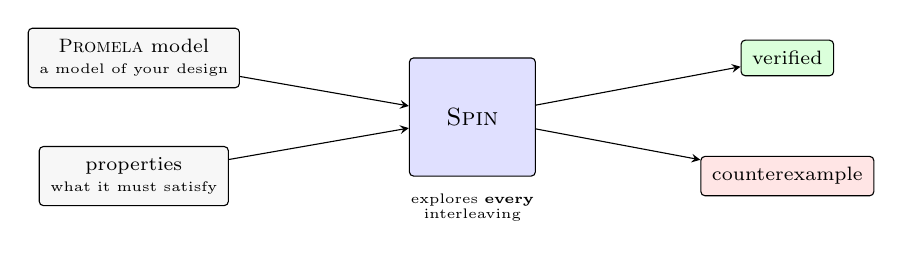
\begin{tikzpicture}[
  font=\scriptsize, >=stealth,
  b/.style={draw, rounded corners=1.5pt, align=center, inner sep=4pt,
            fill=black!3},
  lab/.style={font=\tiny, inner sep=1.5pt}
]
  \node[b] (m) at (0,0.75)  {\promelaname{} model\\{\tiny a model of your design}};
  \node[b] (p) at (0,-0.75) {properties\\{\tiny what it must satisfy}};
  \node[b, fill=blue!12, minimum height=1.5cm, minimum width=1.6cm,
        font=\small\bfseries] (s) at (4.3,0) {\spin{}};
  \node[b, fill=green!14] (ok)  at (8.3,0.75)  {verified};
  \node[b, fill=red!10]   (cex) at (8.3,-0.75) {counterexample};

  \draw[->] (m) -- (s);
  \draw[->] (p) -- (s);
  \draw[->] (s) -- (ok);
  \draw[->] (s) -- (cex);
  \node[lab, align=center] at (4.3,-1.15) {explores {\bf every}\\interleaving};
\end{tikzpicture}\par}

\vspace{0.35cm}

Either it finds no violation in {\em any} interleaving, or it hands back the one
execution that breaks the property.

\pause
\vspace{0.3cm}

\begin{itemize}
\item Developed by {\bf Gerard Holzmann}, originally at Bell Labs, later at JPL.
\item ACM {\bf Software System Award}, 2001.
\item Open source, actively used in industry and at NASA for 30+ years.
\item \url{https://spinroot.com}
\end{itemize}

\end{frame}

        %  2 min
%----------------------------------------
\begin{frame}
  \frametitle{Part 1}

{\Large\bf Motivation: why concurrency defeats testing}

\end{frame}

%----------------------------------------
\begin{frame}[fragile]
  \frametitle{Six lines of obviously correct code} \small

Two instruments share a $10\,$A power bus. Each draws $6\,$A, and each asks the
power manager before switching on.

\begin{lstlisting}[language=promela]
byte avail   = 10;             /* SHARED: amps left on the bus  */
byte powered = 0;              /* SHARED: instruments now on    */

inline request_power(amps) {
  if
  :: avail >= amps ->          /* CHECK: is there enough?       */
       avail = avail - amps;   /* ACT:   reserve it             */
       powered++               /*        switch on              */
  :: else -> skip              /* denied - stay off             */
  fi
}

active proctype InstrumentA() { request_power(6) }   /* thread 1 */
active proctype InstrumentB() { request_power(6) }   /* thread 2 */
\end{lstlisting}

\end{frame}

%----------------------------------------
\begin{frame}
  \frametitle{The interleaving that flies} \small

\begin{center}\scriptsize
\begin{tabular}{c l l r r}
\toprule
{\bf step} & {\bf Instrument A} & {\bf Instrument B} & {\bf avail} & {\bf powered}\\
\midrule
0 & \multicolumn{2}{l}{\em (initial)}                       & 10 & 0\\
1 & \tt avail >= 6 ? yes  &                                 & 10 & 0\\
\rowcolor{red!8}
2 &                       & \tt avail >= 6 ? yes            & 10 & 0\\
3 & \tt avail = 10 - 6    &                                 &  4 & 0\\
4 & \tt powered++         &                                 &  4 & 1\\
5 &                       & \tt avail = 4 - 6               & \bf 254 & 1\\
6 &                       & \tt powered++                   & \bf 254 & \bf 2\\
\bottomrule
\end{tabular}
\end{center}

\pause
\vspace{0.3cm}

\begin{block}{Two failures for the price of one}\small
\begin{itemize}
\item {\bf $12\,$A drawn from a $10\,$A bus.} Brownout, undervoltage trip, or a
      reset --- on hardware, not in the model.
\item {\bf \ipromela{avail} underflowed} $4-6 = -2$, and as a \ipromela{byte} that is
      $254$. The power manager now believes it has $254\,$A to give away.
      {\em Every subsequent request succeeds.}
\end{itemize}
\end{block}

\pause

The second failure is the dangerous one: the system does not crash here.
It quietly stops enforcing the budget, and fails somewhere else, much later.

\end{frame}

%----------------------------------------
\begin{frame}
  \frametitle{Why testing does not find this} \small

The window is {\bf two instructions wide} --- it needs a preemption landing
exactly between the check and the act.

\pause
\vspace{0.4cm}

\begin{block}{}\small
\centering
The defect is in the {\bf interleaving}. Reviewing interleavings is\\
far harder than reviewing sequential behavior.
\end{block}

\end{frame}

%----------------------------------------
\begin{frame}
  \frametitle{The number of interleavings explodes} \small

$n$ tasks, each with $m$ atomic steps, gives

\[
\frac{(n \cdot m)!}{(m!)^n}
\]

distinct interleavings.

\vspace{0.15cm}

\begin{center}
\begin{tabular}{r r r}
\toprule
{\bf tasks} & {\bf steps each} & {\bf interleavings}\\
\midrule
2 &  2 & 6 \\
3 &  3 & 1\,680 \\
4 &  4 & 63\,063\,000 \\
5 &  5 & $\approx 6.2 \times 10^{14}$ \\
\rowcolor{red!8}
6 &  6 & $\approx 2.7 \times 10^{24}$ \\
\bottomrule
\end{tabular}
\end{center}

\pause
\vspace{0.1cm}

\begin{columns}[c]
\begin{column}{0.36\textwidth}
\centering
\starfield[0.74]
\end{column}
\begin{column}{0.60\textwidth}\small
Six tasks of six steps have more interleavings than there are
{\bf stars in the observable universe} ($\approx 2 \times 10^{23}$).

\vspace{0.25cm}
\pause
This is the famous {\bf state explosion problem}, and it is the
central obstacle for model checking. We return to it later.
\end{column}
\end{columns}

\end{frame}

% ===== HIDDEN 2026-09-09 at Klaus's request: Mars Pathfinder, 1997 =====
%%----------------------------------------
%\begin{frame}
%  \frametitle{Mars Pathfinder, 1997} \small
%
%Repeated total system resets on the surface of Mars.
%
%\vspace{0.25cm}
%
%\begin{block}{Priority inversion}\small
%A {\bf low}-priority meteorological task held a mutex on the information bus.
%A {\bf high}-priority bus-management task blocked on that mutex.
%A {\bf medium}-priority communications task then preempted the low-priority one.
%The mutex was never released, the high-priority task missed its deadline, and
%the watchdog reset the spacecraft.
%\end{block}
%
%\pause
%\vspace{0.25cm}
%
%{\bf Why the medium task matters.} Without it the blocking is bounded by the
%{\em length of the critical section}. The medium task starves the holder, so the
%blocking is bounded only by how long an {\em unrelated} task chooses to run.
%
%\pause
%\vspace{0.25cm}
%
%{\bf Why it is hard to find.} The medium task {\em never touches the mutex}.
%It appears in no analysis of that lock, and reviewing the two tasks that share
%it reveals nothing. The fault is not in any component --- it is in the global
%interleaving of three.
%
%\pause
%\vspace{0.25cm}
%
%Fixed in flight by enabling {\bf priority inheritance} on that mutex.
%
%\end{frame}

%----------------------------------------
\begin{frame}
  \frametitle{The idea of model checking} \small

\begin{block}{}\small
A model checker takes a {\bf finite-state model} $M$ and a {\bf property} $\varphi$,
and decides whether
\[
M \models \varphi
\]
If not, it returns a {\bf counterexample}: a concrete execution that violates $\varphi$.
\end{block}

\pause
\vspace{0.3cm}

\begin{center}\small
\renewcommand{\arraystretch}{1.25}
\begin{tabular}{|l|p{3.5cm}|p{3.9cm}|}
\hline
\rowcolor{blue!10}
& {\bf Testing} & {\bf Model checking}\\
\hline
{\bf What runs}  & The real system        & A model of the system\\
\hline
{\bf Coverage}   & One execution per test & All executions\\
\hline
{\bf Guarantee}  & Finds bugs, cannot prove absence & Proves absence, within the model\\
\hline
{\bf Scale}      & Full systems           & Limited by the state space\\
\hline
{\bf Effort}     & No model needed        & A model must be built\\
\hline
\end{tabular}
\end{center}

\end{frame}
     %  6 min   Part 1
%----------------------------------------
\begin{frame}
  \frametitle{Part 2}

{\Large\bf \promelaname{}: the modeling language}

\end{frame}

%----------------------------------------
\begin{frame}
  \frametitle{\promelaname{} in one slide} \small

{\em Process Meta Language}. C-like syntax, but it is a {\bf modeling} language,
not a programming language.

\vspace{0.3cm}

\begin{itemize}
\item {\bf Processes} (\ipromela{proctype}) --- the units of concurrency.
\item {\bf Channels} (\ipromela{chan}) --- synchronous or buffered message passing.
\item {\bf Global and local variables} --- finite types only (\ipromela{bit}, \ipromela{byte}, \ipromela{short}, \ipromela{int}, \ipromela{mtype}).
\item {\bf Guarded commands} --- \ipromela{if}/\ipromela{fi} and \ipromela{do}/\ipromela{od}, with nondeterministic choice.
\item {\bf Blocking semantics} --- a statement executes only when it is {\em executable}.
\end{itemize}

\pause
\vspace{0.3cm}

\begin{block}{Important idea}\small
In \promelaname{} a {\bf boolean expression is a statement}. It blocks until it is
true. So \ipromela{(x > 0)} on its own line means ``wait until \ipromela{x > 0}''.
\end{block}

\end{frame}

%----------------------------------------
\begin{frame}[fragile]
  \frametitle{Processes} \small

\begin{lstlisting}[language=promela]
byte powered = 0;              /* global, shared */

proctype Instrument(byte id) {
  byte local = 0;              /* local to each instance */
  local = powered;
  powered = local + 1;
  printf("instrument %d on\n", id)
}

init {
  run Instrument(1);           /* spawn */
  run Instrument(2)
}
\end{lstlisting}

\pause

Statements of different processes interleave arbitrarily --- {\bf that is the
point}.

\end{frame}

%----------------------------------------
\begin{frame}[fragile]
  \frametitle{Guarded commands: \tool{if}} \small

\begin{lstlisting}[language=promela]
/* the environment: temperature does what it likes */
if
:: (t < 120) -> t = t + 10        /* it rises           */
:: (t >   0) -> t = t - 10        /* it falls           */
:: true      -> sensor = FAILED   /* or the sensor dies */
fi
\end{lstlisting}

\pause
\vspace{0.2cm}

\begin{block}{Semantics}\small
\begin{itemize}
\item Every guard is evaluated. {\bf All} true guards are candidates.
\item One of them is chosen {\bf nondeterministically}. For $0 < t < 120$ all
      three hold, and \spin{} explores {\bf all three} branches.
\item Guard order is irrelevant --- this is not C's \tool{else if}.
\item If no guard is true and there is no \ipromela{else}, the \ipromela{if} {\bf blocks}.
\end{itemize}
\end{block}

\pause
\vspace{0.2cm}

{\bf Nondeterminism is a modeling tool}, not a bug. No branch here is the
``right'' one: whatever you prove holds for {\em every} environment behavior,
including the sensor failing at the worst possible moment.

\end{frame}

%----------------------------------------
\begin{frame}[fragile]
  \frametitle{Guarded commands: \tool{do}} \small

\begin{lstlisting}[language=promela]
/* the same environment, now running forever */
do
:: (t < 120) -> t = t + 10
:: (t >   0) -> t = t - 10
:: true      -> sensor = FAILED; break
od
\end{lstlisting}

\vspace{0.2cm}

Same choice rule, repeated forever until \ipromela{break} or \ipromela{goto}.
The temperature now wanders over every reachable value, and the sensor may fail
at {\bf any} point along the way.

\end{frame}

%----------------------------------------
\begin{frame}[fragile]
  \frametitle{Channels} \small

\begin{lstlisting}[language=promela]
mtype = { HEAT, COOL, ACK };          /* symbolic constants */

chan cmd  = [0] of { mtype, byte };   /* rendezvous  */
chan tlm  = [8] of { mtype, byte };   /* buffered, capacity 8 */

cmd ! HEAT, 42;      /* send    */

mtype msg; byte value;
tlm ? msg, value;    /* receive */
\end{lstlisting}

\pause
\vspace{0.2cm}

\begin{itemize}
\item Capacity \ipromela{[0]} $\Rightarrow$ {\bf synchronous} handshake: sender and
      receiver move together.
\item Capacity $>0$ $\Rightarrow$ {\bf asynchronous} FIFO; send blocks when full,
      receive blocks when empty.
\item \ipromela{len(ch)}, \ipromela{empty(ch)}, \ipromela{full(ch)}, \ipromela{nempty(ch)}, \ipromela{nfull(ch)}.
\item \ipromela{ch ? eval(x)} matches only a message equal to the current value of \ipromela{x};
      \ipromela{ch ? [msg, value]} tests receivability without consuming.
\end{itemize}

\end{frame}

%----------------------------------------
\begin{frame}[fragile]
  \frametitle{Modeling an unreliable channel} \small

\begin{lstlisting}[language=promela]
do
:: link ? msg ->
     if
     :: out ! msg              /* delivered    */
     :: skip                   /* silently lost */
     :: out ! msg; out ! msg   /* duplicated   */
     fi
od
\end{lstlisting}

\vspace{0.25cm}

{\centering
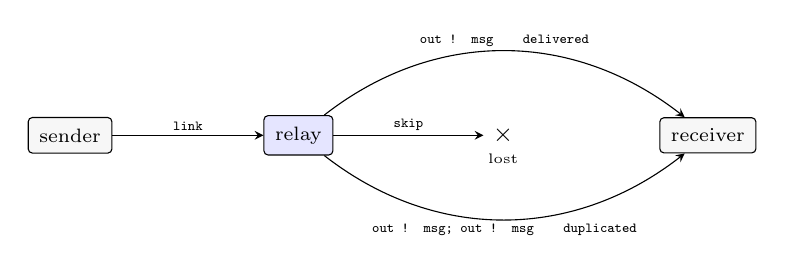
\begin{tikzpicture}[
  font=\scriptsize, >=stealth,
  b/.style={draw, rounded corners=1.5pt, align=center, inner sep=4pt,
            fill=black!3},
  lab/.style={font=\tiny, inner sep=1.5pt}
]
  \node[b] (s) at (0,0)                  {sender};
  \node[b, fill=blue!10] (r) at (2.9,0)  {relay};
  \node[b] (d) at (8.1,0)                {receiver};

  \draw[->] (s) -- node[lab, above] {\tt link} (r);

  \draw[->] (r) to[out=38,in=142]
        node[lab, above] {\tt out ! msg \ \ \ delivered} (d);
  \node[font=\small] (x) at (5.5,0) {$\times$};
  \draw[->] (r) -- node[lab, above] {\tt skip} (x);
  \node[lab] at (5.5,-0.3) {lost};
  \draw[->] (r) to[out=-38,in=-142]
        node[lab, below] {\tt out ! msg; out ! msg \ \ \ duplicated} (d);
\end{tikzpicture}\par}

\pause
\vspace{0.25cm}

Three lines of nondeterminism replace an entire fault-injection harness.
Every property you then prove holds under loss and duplication.

\end{frame}

%----------------------------------------
\begin{frame}[fragile]
  \frametitle{Atomicity} \small

By default, {\bf every statement is a possible preemption point}.
Two ways to say otherwise:

\vspace{0.3cm}

\begin{lstlisting}[language=promela]
atomic { t = x; x = t + 1 }   /* atomicity lost if it blocks */

d_step { t = x; x = t + 1 }   /* one step, may never block  */
\end{lstlisting}

\pause
\vspace{0.3cm}

\begin{block}{Why you care}\small
\begin{itemize}
\item \ipromela{atomic} and \ipromela{d_step} are how you model a critical section,
      a disabled-interrupt region, or a hardware-atomic instruction.
\item They are also the main lever for {\bf reducing the state space}: fewer
      interleaving points means exponentially fewer states.
\item {\bf Danger:} over-using them hides the very bugs you are looking for.
\end{itemize}
\end{block}

\end{frame}

        % 10 min   Part 2
%----------------------------------------
\begin{frame}
  \frametitle{Part 3}

{\Large\bf Stating properties}

\end{frame}

%----------------------------------------
\begin{frame}
  \frametitle{Two kinds of property} \small

\begin{block}{Safety --- ``nothing bad ever happens''}\small
Violated by a {\bf finite} execution prefix.\\
{\em Both instruments powered simultaneously. An assertion fails. A deadlock.}
\end{block}

\pause

\begin{block}{Liveness --- ``something good eventually happens''}\small
Violated only by an {\bf infinite} execution.\\
{\em A request is never granted. The system loops forever without progressing.}
\end{block}

\pause
\vspace{0.4cm}

\spin{} handles both, but by different machinery:
safety by ordinary reachability, liveness by cycle detection.
Liveness checking is roughly twice the cost.

\end{frame}

%----------------------------------------
\begin{frame}[fragile]
  \frametitle{Level 1: assertions} \small

\begin{lstlisting}[language=promela]
assert(powered <= 1);
assert(len(cmd_queue) < QUEUE_MAX);
assert(mode != SAFE_MODE || thrusters_off);
\end{lstlisting}

\pause
\vspace{0.3cm}

\begin{block}{Global invariants}\small
Put the invariant in its own monitor process; \spin{} will interleave it everywhere:
\begin{lstlisting}[language=promela]
active proctype Monitor() {
  assert(powered <= 1)      /* checked at all interleaving points */
}
\end{lstlisting}
\end{block}

\end{frame}

%----------------------------------------
\begin{frame}[fragile]
  \frametitle{Level 2: end states, progress, acceptance} \small

\begin{block}{Valid end states --- \ipromela{end} labels}\small
By default a process must terminate to end validly. Label a legitimate blocking
point to say ``stopping here is fine'':
\begin{lstlisting}[language=promela]
end_wait: do :: cmd ? c -> handle(c) od
\end{lstlisting}
Without the \ipromela{end} prefix, an idle server looks like a deadlock.
\end{block}

\pause

\begin{block}{Progress --- \ipromela{progress} labels}\small
\begin{lstlisting}[language=promela]
progress_grant: powered++;
\end{lstlisting}
With \tool{./pan -l}, \spin{} reports any infinite execution that does {\bf not}
pass a \ipromela{progress} label infinitely often --- i.e.\ livelock / starvation.
\end{block}

\end{frame}

%----------------------------------------
\begin{frame}[fragile]
  \frametitle{Level 3: Linear Temporal Logic} \small

Over an infinite execution $\sigma = s_0 s_1 s_2 \ldots$

\vspace{0.3cm}

\begin{center}
\begin{tabular}{l l p{5.0cm}}
\toprule
{\bf Operator} & {\bf \spin{} syntax} & {\bf Meaning}\\
\midrule
$\LTLsquare\, p$          & \verb|[] p|      & $p$ holds in every state\\
$\LTLdiamond\, p$         & \verb|<> p|      & $p$ holds in some future state\\
$\Next\, p$               & \verb|X p|       & $p$ holds in the next state\\
$p \until q$              & \verb|p U q|     & $p$ holds until $q$ holds, and $q$ does\\
\bottomrule
\end{tabular}
\end{center}

\pause
\vspace{0.4cm}

\begin{block}{The three patterns that cover most real requirements}\small
\begin{tabular}{l l}
{\bf Invariance} & $\LTLsquare\, \neg bad$ \\[0.1cm]
{\bf Response}   & $\LTLsquare\, (request \rightarrow \LTLdiamond\, grant)$ \\[0.1cm]
{\bf Precedence} & $\neg action \until authorization$ \\
\end{tabular}
\end{block}

\end{frame}

%----------------------------------------
\begin{frame}[fragile]
  \frametitle{LTL in \promelaname{}} \small

\begin{lstlisting}[language=promela]
#define p0  (want[0])          /* instrument 0 requests */
#define g0  (powered_by == 0)  /* instrument 0 has the bus */
#define mutex (powered <= 1)

ltl safety   { [] mutex }
ltl response { [] (p0 -> <> g0) }
ltl no_starve { []<> g0 }
\end{lstlisting}

\end{frame}

% ===== HIDDEN 2026-09-09 at Klaus's request: Never claims and trace assertions =====
%%----------------------------------------
%\begin{frame}[fragile]
%  \frametitle{Never claims and \tool{trace} assertions} \small
%
%\begin{block}{Never claim --- the automaton \spin{} actually runs}\small
%An \ipromela{ltl} formula is compiled into a \ipromela{never} claim: a \buchi{}
%automaton describing the {\bf violating} behaviors. You can also write one by hand.
%\end{block}
%
%\pause
%
%\begin{lstlisting}[language=promela]
%/* the violations of  ltl no_starve { []<> g0 },     */
%/* which are the runs satisfying  <>[] !g0           */
%never {
%T0_init:
%  do
%  :: true                    /* not yet committed          */
%  :: !g0 -> goto accept_S    /* guess: g0 never holds again */
%  od;
%accept_S:
%  do :: !g0 od               /* and it never does           */
%}
%\end{lstlisting}
%
%\pause
%\vspace{0.15cm}
%
%The \ipromela{accept_} label is what makes it liveness: a violation is an infinite
%run through it. Make \ipromela{T0_init} accepting too and the claim matches
%{\em every} run.
%
%\pause
%
%\ipromela{trace} / \ipromela{notrace} assertions instead constrain the {\bf order
%of channel operations} across the whole system.
%
%\end{frame}
     %  8 min   Part 3
%%----------------------------------------
\begin{frame}
  \frametitle{Part 4}

{\Large\bf Worked examples}

\vspace{0.5cm}

{\large 1. Mutual exclusion --- a shared instrument}

\end{frame}

%----------------------------------------
\begin{frame}
  \frametitle{The system: a shared instrument} \small

\begin{block}{Informal requirements}\small
Two science instruments share a single power bus. Each must acquire the bus
before drawing power and release it afterwards.

\begin{enumerate}
\item {\bf Safety:} the two instruments are never powered simultaneously.
\item {\bf Liveness:} an instrument requesting power eventually gets it.
\item {\bf No deadlock:} the system never wedges.
\end{enumerate}
\end{block}

\pause
\vspace{0.3cm}

This is mutual exclusion. It is also, structurally, the Pathfinder bug,
the RTOS mutex, and half the concurrency in any flight system.

\end{frame}

%----------------------------------------
\begin{frame}[fragile]
  \frametitle{Attempt 1: a naive flag protocol} \small

\begin{lstlisting}[language=promela]
bool want[2];       /* want[i]: instrument i requests the bus */
byte powered = 0;   /* number of instruments currently powered */

active [2] proctype Instrument() {
  byte me = _pid;
  do
  :: want[me] = true;
     (!want[1-me]);          /* wait until the other is not asking */
     powered++;              /* CRITICAL: drawing power */
     assert(powered == 1);
     powered--;
     want[me] = false
  od
}
\end{lstlisting}

\pause

\begin{itemize}
\item \ipromela{_pid} is the process instance number, $0$ and $1$ here.
\item \ipromela{(!want[1-me])} is a {\bf blocking wait}, not an \ipromela{if}.
\item \ipromela{assert} states the safety requirement inline.
\end{itemize}

\end{frame}

%----------------------------------------
\begin{frame}[fragile]
  \frametitle{What \spin{} says} \small

\begin{lstlisting}[style=shell]
$ spin -a instrument.pml
$ gcc -o pan pan.c
$ ./pan

pan:1: invalid end state (at depth 4)
pan: wrote instrument.pml.trail

State-vector 20 byte, depth reached 5, errors: 1
\end{lstlisting}

\pause
\vspace{0.3cm}

\begin{block}{The counterexample --- a deadlock}\small
\begin{enumerate}
\item Instrument 0 sets \ipromela{want[0] = true}.
\item Instrument 1 sets \ipromela{want[1] = true}.
\item Instrument 0 blocks waiting for \ipromela{!want[1]}.
\item Instrument 1 blocks waiting for \ipromela{!want[0]}.
\end{enumerate}
Both are stuck. \spin{} found it at {\bf depth 4}, in milliseconds.
\end{block}

\pause

Note: the \ipromela{assert} never fired. Safety held; {\em progress} did not.

\end{frame}

%----------------------------------------
\begin{frame}[fragile]
  \frametitle{Attempt 2: Peterson's algorithm} \small

\begin{lstlisting}[language=promela]
bool want[2];
byte turn;
byte powered = 0;

active [2] proctype Instrument() {
  byte me = _pid;
  do
  :: want[me] = true;
     turn = 1 - me;                       /* politely defer */
     (!want[1-me] || turn == me);         /* wait */
     powered++;
     assert(powered == 1);                /* mutual exclusion */
     powered--;
     want[me] = false
  od
}
\end{lstlisting}

\pause
\vspace{0.2cm}

\begin{lstlisting}[style=shell]
$ ./pan
State-vector 20 byte, depth reached 27, errors: 0
\end{lstlisting}

{\bf Verified:} no assertion violation and no deadlock, over {\em all} interleavings.

\end{frame}
      %  6 min   HIDDEN 2026-09-08 -- Peterson/mutual exclusion
%----------------------------------------
\begin{frame}
  \frametitle{Part 4}

{\Large\bf Worked examples}

\vspace{0.5cm}

{\large 1. A recent analysis}

\vspace{0.25cm}

{\small A lock-free priority queue, August 2026}

\end{frame}

%----------------------------------------
\begin{frame}[fragile]
  \frametitle{The queue} \small

\begin{block}{The problem}\small
A message queue built on a mutex cannot be used from an interrupt handler, because
a mutex cannot be taken there.
\end{block}

\vspace{0.15cm}

So: replace the mutex with compare-and-swap.

\vspace{0.15cm}

An array of \tool{depth} {\bf slots}. Each holds one message and an atomic word
giving its state --- all \ipromela{FREE} to begin with:

\vspace{0.25cm}

{\centering
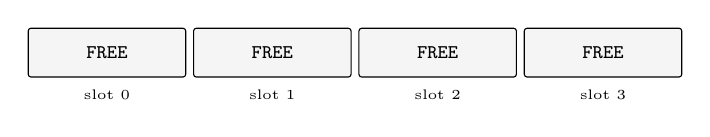
\begin{tikzpicture}
  \foreach \i in {0,1,2,3} {
    \draw[fill=black!4, rounded corners=1pt] (\i*2.1,0) rectangle (\i*2.1+2.0,0.62);
    \node[font=\scriptsize\ttfamily] at (\i*2.1+1.0,0.31) {FREE};
    \node[font=\tiny] at (\i*2.1+1.0,-0.22) {slot \i};
  }
\end{tikzpicture}\par}

\vspace{0.3cm}

{\centering\small
\ipromela{FREE} $\to$ \ipromela{WRITING} $\to$ \ipromela{READY} $\to$
\ipromela{READING} $\to$ \ipromela{FREE}\par}

\vspace{0.25cm}

A producer takes a slot by winning the CAS \ipromela{FREE}$\to$\ipromela{WRITING};
a consumer takes it by winning the CAS \ipromela{READY}$\to$\ipromela{READING}. {\bf Winning
the CAS is what confers ownership} --- two consumers may pick the same slot, only
one wins, so nothing is delivered twice.

\end{frame}

%----------------------------------------
\begin{frame}[fragile]
  \frametitle{And one counter, purely for speed} \small

Scanning the whole array every time, just to see whether there is an element, is
costly --- and it is asked every dispatch cycle.

\pause
\vspace{0.35cm}

\begin{block}{The optimization: \tool{available}}\small
A counter, so a consumer can skip the scan when there are likely no elements.

\vspace{0.15cm}

The count now lives in {\bf two places} --- the counter, and implicitly the slots
themselves. They need not match exactly: the counter is only a hint, and whoever
passes it still runs the real scan. What matters is {\em which way} it is allowed
to be wrong.

\vspace{0.15cm}

It is also public: \tool{getMessagesAvailable()} is downlinked as telemetry.
\end{block}

\end{frame}

%----------------------------------------
\begin{frame}[fragile]
  \frametitle{\tool{send} and \tool{receive}, as written} \small

\begin{lstlisting}[style=shell]
send(m):
    slot = claimFreeSlot()               # CAS FREE -> WRITING
    write(slot, m)
    publish(slot)                        # CAS WRITING -> READY
    available += 1                       # credit it AFTER publishing

receive():
    repeat, at most MAX_RETRY_PASSES times:   # a pass = peek, scan, claim
        if available == 0:      continue      # 1. peek: skip the scan
        slot = selectBestReady()              # 2. scan: claims nothing
        if slot == none:        continue
        if CAS(slot, READY -> READING):       # 3. claim: fails if another
            available -= 1                    #    consumer got there first
            m = read(slot)
            release(slot)                     # CAS READING -> FREE
            return m
        # lost the claim -- yield and try again
    return EMPTY                              # all passes used up
\end{lstlisting}

\pause

No mutex means nothing to sleep on: a blocking caller {\bf polls} the counter, not
the array.

\pause

Only the third step commits to anything: the decrement is authorized by {\bf
winning that CAS}. Two consumers winning on {\em different} slots have both earned
one.

\end{frame}

%----------------------------------------
\begin{frame}[fragile]
  \frametitle{The model --- the producer} \small

Claude Code flagged an issue. I then asked it to generate a \promelaname{} model
to illustrate it.

\begin{lstlisting}[language=promela]
/* FREE=0, WRITING=1, READY=2, READING=3 */
byte slot[2] = FREE;              /* each slot's state */
int  avail = 0;                   /* signed: underflow shows as -1 */
active [2] proctype Producer() {
  int myslot;                     /* the slot this producer claimed */
  do
  :: atomic {                     /* the claim CAS */
       if
       :: (slot[0] == FREE) -> slot[0] = WRITING; myslot = 0
       :: (slot[1] == FREE) -> slot[1] = WRITING; myslot = 1
       fi
     }
     if
     :: (myslot == 0) -> slot[0] = READY
     :: (myslot == 1) -> slot[1] = READY
     fi;
     avail++                      /* publish, THEN credit */
  od
}
\end{lstlisting}

\end{frame}

%----------------------------------------
\begin{frame}[fragile]
  \frametitle{The model --- the consumer} \small

\begin{lstlisting}[language=promela]
active [2] proctype Consumer() {
  int myslot;                     /* -1 if nothing was claimed */
  do
  :: avail > 0 ->                 /* the peek: a step of its own */
     atomic {                     /* the claim CAS */
       if
       :: (slot[0] == READY) -> slot[0] = READING; myslot = 0; avail--
       :: (slot[1] == READY) -> slot[1] = READING; myslot = 1; avail--
       :: else               -> myslot = -1
       fi
     }
     assert(avail >= 0);
     if
     :: (myslot ==  0) -> slot[0] = FREE    /* release: READING -> FREE */
     :: (myslot ==  1) -> slot[1] = FREE
     :: (myslot == -1) -> skip              /* claimed nothing */
     fi
  od
}
\end{lstlisting}

Two producers, two consumers, two slots; of a slot, only its {\bf state} is
modelled.

\pause

The crux: publish and \ipromela{avail++} are separate statements, and so are the
peek and the claim. Put either pair inside one \ipromela{atomic} and the bug
vanishes.

\end{frame}

%----------------------------------------
\begin{frame}[fragile]
  \frametitle{What \spin{} says} \small

\begin{lstlisting}[style=shell]
pan:1: assertion violated (avail>=0) (at depth 11)
\end{lstlisting}

\vspace{0.1cm}

{\centering\scriptsize
\begin{tabular}{rlll}
\toprule
{\bf step} & {\bf proc} & {\bf action} & {\bf avail} \\
\midrule
 1 & P  & claim slot 0                      & 0 \\
 3 & P  & publish slot 0 $\to$ \ipromela{READY} & 0 \\
 4 & P  & \tool{avail++}                    & 1 \\
 5 & C1 & peek: \tool{avail > 0}, pass      & 1 \\
 6 & C2 & peek: \tool{avail > 0}, pass      & 1 \\
 7 & C1 & claim slot 0, \tool{avail-\/-}      & 0 \\
 8 & P  & claim slot 1                      & 0 \\
10 & P  & publish slot 1 --- {\em uncredited} & 0 \\
11 & C2 & claim slot 1, \tool{avail-\/-}      & {\bf $-1$} \\
12 & \multicolumn{2}{l}{\ipromela@assert(avail >= 0)@ fails} & \\
\bottomrule
\end{tabular}\par}

\pause
\vspace{0.2cm}

Both consumers won a claim, on {\em different} slots, so both were entitled to
decrement --- but only one credit had landed. The real field is \tool{unsigned}:
telemetry reads {\bf 4\,294\,967\,295}.

\pause

Mirror symptom, same gap: the peek reads $0$ past a published message, so a
non-blocking \tool{receive} runs out its passes and returns \tool{EMPTY} with the
queue non-empty --- a {\bf linearizability violation}.

\end{frame}

%----------------------------------------
\begin{frame}[fragile]
  \frametitle{The fix} \small

\begin{lstlisting}[style=shell]
send(m):
    slot = claimFreeSlot()
    write(slot, m)
    available += 1              # credit it BEFORE publishing
    publish(slot)               # CAS WRITING -> READY
\end{lstlisting}

\vspace{0.1cm}

Every decrement is now preceded by its own credit, so underflow is unreachable
--- and \tool{available == 0} soundly implies no slot is \ipromela{READY}, which
kills the spurious \tool{EMPTY} too.

\vspace{0.2cm}

\begin{lstlisting}[style=shell]
State-vector 48 byte, depth reached 1097, errors: 0
     1992 states, stored
\end{lstlisting}

\pause
\vspace{0.15cm}

\begin{block}{The trade-off, stated honestly}\small
With two racing atomics you cannot have both {\em never over-report} and {\em
never underflow}. Crediting first over-reports by at most \tool{depth} --- benign,
because the peek was only ever a hint: a consumer that passes it still runs the
real scan, finds nothing, and gives up.
\end{block}

\end{frame}

%----------------------------------------
\begin{frame}
  \frametitle{Why the tests did not catch it} \small

\begin{itemize}
\item The author's tests pass: {\bf 29/29} functional, {\bf 15/15} under
      ThreadSanitizer, {\bf zero} race reports.
\item It {\em is} a race --- but a {\bf high-level} one, across two variables:
      the publish and the credit. Not a data race on one location. Every
      individual access is a properly synchronized atomic, so ThreadSanitizer
      has nothing to see.
\item The stress tests assert exactly-once delivery, which genuinely holds.
      Nothing asserted \tool{available} $\leq$ \tool{depth}.
\end{itemize}

\pause
\vspace{0.3cm}

\begin{block}{The part worth pausing on}\small
\tool{available} did not exist in the original PR. It was {\em added} to fix an
earlier reviewer's finding --- and the ordering that reviewer recommended,
faithfully implemented, is the ordering that underflows.

\vspace{0.15cm}

The fix for the first problem created this one.
\end{block}

\end{frame}
       %  5 min   Part 4 -- worked example 1
%----------------------------------------
\begin{frame}
  \frametitle{Part 4}

{\Large\bf Worked examples}

\vspace{0.5cm}

{\large 2. The Deep Space 1 Remote Agent}

\vspace{0.25cm}

{\small Havelund, Lowry \& Penix, NASA Ames --- {\em Formal Analysis of a Space
Craft Controller using \spin{}}}

\end{frame}

%----------------------------------------
\begin{frame}
  \frametitle{The system} \small

The {\bf Remote Agent} is an AI-based spacecraft controller: a planner, a plan
{\bf execution module}, and a mode identification and recovery module. It flew on
Deep Space 1, launched October 1998, and in May 1999 controlled a spacecraft
autonomously for the first time in NASA's history.

\pause
\vspace{0.3cm}

We analyzed the executive's bottom layer --- {\bf ESL}, a language built on
multithreaded Common Lisp. Tasks {\em achieve} and {\em maintain} properties of
the spacecraft, take {\bf locks} on them to exclude incompatible tasks, and a
{\bf daemon} watches for a locked property no longer holding.

\pause
\vspace{0.3cm}

\begin{block}{The model}\small
About {\bf 3000 lines} of Lisp, hand-translated to {\bf 500 lines} of
\promelaname{} --- abstracted down to the lock-table operations, with two
property names, two events, and three tasks. Twelve man-weeks to build; about a
week to verify.
\end{block}

\end{frame}

%----------------------------------------
\begin{frame}
  \frametitle{The Remote Agent Executive} \small

\vspace{0.1cm}

{\centering
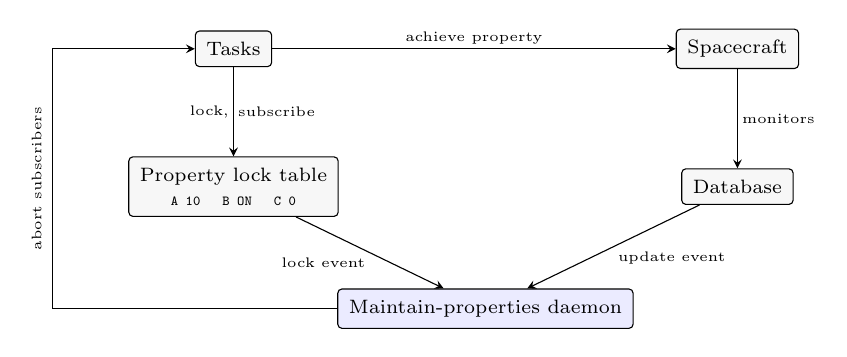
\begin{tikzpicture}[
  font=\scriptsize, >=stealth,
  box/.style={draw, rounded corners=1.5pt, align=center, inner sep=4pt,
              fill=black!3},
  lbl/.style={font=\tiny, inner sep=1.5pt}
]
  \node[box] (tasks) at (0,0)      {Tasks};
  \node[box] (sc)    at (6.4,0)    {Spacecraft};
  \node[box] (locks) at (0,-1.75)  {Property lock table\\[1pt]
        {\tiny\ttfamily A~10 \quad B~ON \quad C~0}};
  \node[box] (db)    at (6.4,-1.75) {Database};
  \node[box, fill=blue!8] (dae) at (3.2,-3.3) {Maintain-properties daemon};

  \draw[->] (tasks) -- node[lbl, above] {achieve property} (sc);
  \draw[->] (sc)    -- node[lbl, right] {monitors} (db);
  \draw[->] (tasks) -- node[lbl, left]  {lock,} node[lbl, right] {subscribe} (locks);
  \draw[->] (locks) -- node[lbl, below left]  {lock event}   (dae);
  \draw[->] (db)    -- node[lbl, below right] {update event} (dae);
  \draw[->] (dae.west) -- (-2.3,-3.3) -- (-2.3,0) -- (tasks.west);
  \node[lbl, rotate=90] at (-2.5,-1.65) {abort subscribers};
\end{tikzpicture}\par}

\pause
\vspace{0.2cm}

A task locks a property, then achieves it --- writing it into the spacecraft. The
{\bf database} is what the monitors actually observe. When the lock table says a
property is held and achieved but the database disagrees, that is an {\bf
inconsistency}, and the daemon must abort every task subscribed to it.

\end{frame}

%----------------------------------------
\begin{frame}[fragile]
  \frametitle{Two properties, written by the programmers} \small

Crucially, the RA programmers formulated these {\em after} the \promelaname{}
model had been written --- so the properties had no influence on the design of the
model, and the model was not built to satisfy them.

\vspace{0.25cm}

\begin{block}{RELEASE}\small
{\em A task releases all of its locks before it terminates.} \\
An assertion, placed after the task's body.
\end{block}

\pause

\begin{block}{ABORT}\small
{\em If an inconsistency occurs between the database and an entry in the lock
table, then all tasks that rely on the lock will be terminated.}
\begin{lstlisting}[language=promela]
[] (task1_property_broken -> <> task1_terminated)
\end{lstlisting}
A {\bf response} property --- the second of the three patterns from Part 3.
\end{block}

\pause
\vspace{0.2cm}

Both turned out to be broken. Five flawed code fragments: one breaking RELEASE,
three breaking ABORT, one efficiency bug. The programmer confirmed all five were
errors in the {\em Lisp}, not just in the model.

\end{frame}

%----------------------------------------
\begin{frame}[fragile]
  \frametitle{Error 2 --- the one that mattered} \small

Three counters:

\vspace{0.1cm}

{\scriptsize
\tool{Ev[MEMORY\_EVENT].count} --- how many times the database has changed.\\
\tool{Ev[LOCK\_EVENT].count} --- how many times the lock table has changed.\\
\tool{event\_count} --- the daemon's snapshot of their sum, last time it looked.\par}

\begin{lstlisting}[language=promela]
if                            /* has anything happened since I looked? */
:: (!first_time &&
    Ev[MEMORY_EVENT].count +
    Ev[LOCK_EVENT].count != event_count) ->
      event_count = Ev[MEMORY_EVENT].count +
                    Ev[LOCK_EVENT].count
:: else ->                    /* no: go to sleep */
      first_time = false;
      /* <-- an event arriving HERE is lost */
      wait_for_events(this, MEMORY_EVENT, LOCK_EVENT)
fi
\end{lstlisting}

\pause

The guard reads the event counters, the \ipromela{else} branch commits to
sleeping --- and the sleeping happens later, as a {\bf separate statement}.

\end{frame}

%----------------------------------------
\begin{frame}[fragile]
  \frametitle{Error 2 --- the fix} \small

\begin{lstlisting}[language=promela]
atomic {                      /* deciding and sleeping, indivisibly */
  if
  :: (!first_time && ...) -> event_count = ...
  :: else -> first_time = false;
             wait_for_events(this, MEMORY_EVENT, LOCK_EVENT)
  fi
}
\end{lstlisting}

\vspace{0.15cm}

One keyword. The daemon can no longer be preempted between deciding that nothing
has happened and going to sleep.

\pause
\vspace{0.3cm}

\begin{block}{}\small
{\em The same shape as the queue.} There it was publish-then-credit; here it is
check-then-wait. Both are a test and the act that depends on it, performed as two
steps --- and in both cases the whole bug is the gap between them.
\end{block}

\end{frame}

%----------------------------------------
\begin{frame}
  \frametitle{18 May 1999} \small

Deep Space 1, 96 million kilometres from Earth. {\bf Thrusting did not turn off
when requested.} The Remote Agent experiment was terminated from the ground and
the spacecraft put into stand-by mode.

\pause
\vspace{0.3cm}

The cause was a deadlock: a missing critical section around a conditional wait,
letting an event arrive between the evaluation of the condition and the wait. The
thread waited, missed the event, and the system wedged.

\pause
\vspace{0.3cm}

\begin{block}{}\small
{\bf The same defect as Error 2} --- and not by coincidence. The code had been
{\bf copied} into another module, and the critical section around it was, by
mistake, left out of the copy. That module was never analyzed with \spin{}.

\vspace{0.15cm}

The repair was to put the critical section back --- the fix \spin{}'s error trace
had already produced, months earlier, for the same pattern elsewhere.
\end{block}

\end{frame}

%----------------------------------------
\begin{frame}
  \frametitle{What the programmer said} \small

On Error 1:

\begin{block}{}\small
{\em ``This is a particularly pernicious bug. It arises only because you are in a
multi-threaded environment, and only in very obscure circumstances that are very
unlikely to arise during testing. Congratulations! You have just converted me into
a believer in formal methods.''}
\end{block}

\pause

On Error 2 --- the pattern that later flew:

\begin{block}{}\small
{\em ``This is an instance of a classic pattern: not wrapping a conditional
wait-for-events inside a critical section. This sort of mistake is very easy to
make and happens all the time in our code. Thanks for catching this one!''}
\end{block}

\pause

Afterwards:

\begin{block}{}\small
{\em ``I used to be very skeptical of the utility of formal methods\dots{} what you
have been doing is finding places where software violates design assumptions,
which is not the same thing as proving correctness. To me you have demonstrated
the utility of this approach beyond any question.''}
\end{block}

\end{frame}
            %  6 min           worked example 2
%----------------------------------------
\begin{frame}
  \frametitle{Part 5}

{\Large\bf How \spin{} works}

\end{frame}

%----------------------------------------
\begin{frame}
  \frametitle{The automata-theoretic approach} \small

\begin{enumerate}
\item The \promelaname{} model is an automaton $A_M$ whose language
      $\mathcal{L}(A_M)$ is the set of all its executions.
\pause
\item The negated property $\neg\varphi$ is translated into a \buchi{} automaton
      $A_{\neg\varphi}$ accepting exactly the {\bf violating} executions.
\pause
\item \spin{} builds the {\bf synchronous product} $A_M \otimes A_{\neg\varphi}$.
\pause
\item Then:
\[
M \models \varphi
\quad\Longleftrightarrow\quad
\mathcal{L}(A_M \otimes A_{\neg\varphi}) = \emptyset
\]
\end{enumerate}

\pause
\vspace{0.4cm}

\begin{block}{}\small
Verification $=$ {\bf emptiness checking}. And a \buchi{} automaton is non-empty
iff some accepting state is reachable {\em and} lies on a cycle.\\[0.2cm]
So: {\bf safety} $=$ find a bad state. {\bf Liveness} $=$ find a bad cycle.
\end{block}

\end{frame}

%----------------------------------------
\begin{frame}
  \frametitle{The search} \small

\begin{block}{Safety: depth-first reachability}\small
Push the initial state; expand successors; hash each into a table; report an error
the first time an assertion fails, an end state is invalid, or a deadlock occurs.
The DFS stack {\bf is} the counterexample.
\end{block}

\pause

\begin{block}{Liveness: a second search, hunting for a loop}\small
A liveness violation is an {\em infinite} bad run --- and in a finite model, an
infinite run means a {\bf loop}. The property automaton marks a state
{\em accepting} when the violation is under way and could go on forever --- for
\ipromela@[]<> g0@ that is ``\ipromela{g0} has not held since''.
So search as usual, and each time you finish exploring an accepting state, start a
{\bf second} search from it asking one question: {\em can I get back here?} If it
can, that loop {\em is} the counterexample.\\[0.15cm]
The {\em nested} depth-first search: linear time, two bits per state --- seen by
the first, seen by the second.
\end{block}

\pause
\vspace{0.15cm}

{\bf On-the-fly:} \spin{} never builds the state graph first --- it constructs
states as it searches and stops at the first violation. A bug in a
$10^{20}$-state system can surface after $10^3$ states.

\end{frame}

%----------------------------------------
\begin{frame}
  \frametitle{The enemy: state explosion} \small

The number of states is roughly

\[
|S| \;\approx\; \prod_{i} |P_i| \;\times\; \prod_{j} |V_j| \;\times\; \prod_{k} |C_k|
\]

--- process locations $\times$ variable valuations $\times$ channel contents.

\pause
\vspace{0.3cm}

{\bf Everything is multiplicative.} One extra \ipromela{byte} variable multiplies
the state space by up to 256. One extra process multiplies it by that process's
entire local state space.

\pause
\vspace{0.4cm}

\begin{block}{Practical implication}\small
Model-checking effort is dominated not by writing \promelaname{} but by
{\bf choosing what to leave out}.
\end{block}

\end{frame}

%----------------------------------------
\begin{frame}
  \frametitle{\spin{}'s weapons against state explosion} \small

\begin{itemize}
\item {\bf Skip the orders that cannot matter} ({\em partial-order reduction}, on
      by default). If two processes are doing things that cannot affect each
      other, try one order and not the other. Usually an order of magnitude, free.
\item {\bf Pack each state tighter} (\tool{-DCOLLAPSE}). Slower, smaller, exact.
\item {\bf Do not keep the states --- keep hashes of them.} One idea at two
      settings; either can miss a bug, neither can invent one.
  \begin{itemize}\small
  \item a {\bf fingerprint} per state (\tool{-DHC}): a few bytes each, so memory
        still grows with the number of states. Errs only if two states collide.
  \item {\bf no entries at all} (\tool{-DBITSTATE}): one fixed-size scoreboard ---
        tick a few boxes per state, ``already ticked'' means ``been here''. A few
        bits rather than 384, whatever the state's size. Errs once other states
        have ticked those boxes between them.
  \end{itemize}
\item {\bf Search in parallel} (\tool{-DNCORE=N}, {\em swarm}): many short searches,
      each looking elsewhere. Good at finding bugs; not a proof.
\item {\bf Give up past a chosen depth} (\tool{-mN}). If the run reports
      \tool{depth reached} equal to your bound it never finished, and
      \tool{errors: 0} means nothing.
\end{itemize}

\pause

{\bf Rule of thumb:} exhaustive if it fits; otherwise a lossy search that finds the
bug beats an exhaustive one that runs out of memory.

\end{frame}
     %  6 min   Part 5
%----------------------------------------
\begin{frame}
  \frametitle{Part 6}

{\Large\bf Using the tool}

\end{frame}

%----------------------------------------
\begin{frame}[fragile]
  \frametitle{The workflow} \small

\begin{lstlisting}[style=shell]
# 1. Sanity: random simulation, watch it run
spin model.pml

# 2. Generate the verifier (C source, specialized to this model)
spin -a model.pml                   # produces pan.c, pan.h, ...

# 3. Compile it
gcc -O2 -o pan pan.c

# 4. Verify
./pan                               # safety: assertions, deadlock
./pan -a                            # + liveness / acceptance cycles
./pan -a -f                         # + weak fairness
./pan -l                            # non-progress cycles

# 5. Replay the counterexample
spin -t -p -l -g model.pml
\end{lstlisting}

\pause
\vspace{0.2cm}

{\bf The key insight:} \spin{} is a {\em verifier generator}. It emits a C program
tailored to your model, which is why it is fast.

\end{frame}

%----------------------------------------
\begin{frame}[fragile]
  \frametitle{Reading the output} \small

\begin{lstlisting}[style=shell]
(Spin Version 6.5.2)
        + Partial Order Reduction

Full statespace search for:
        never claim             - (none specified)
        assertion violations    +
        acceptance   cycles     - (not selected)
        invalid end states      +

State-vector 44 byte, depth reached 178, errors: 0
      1897 states, stored
       912 states, matched
      2809 transitions (= stored+matched)
         0 atomic steps
hash conflicts:         0 (resolved)

Stats on memory usage (in Megabytes):
    0.130       equivalent memory usage for states
  128.195       total actual memory usage
\end{lstlisting}

\end{frame}

%----------------------------------------
\begin{frame}[fragile]
  \frametitle{Reading a counterexample trail} \small

\begin{lstlisting}[style=shell]
$ spin -t -p lockless.pml                              (abridged)

  4: proc 1 (Producer:1) lockless.pml:68 (state 16) [avail = (avail+1)]
  5: proc 3 (Consumer:1) lockless.pml:76 (state 1)  [((avail>0))]
  6: proc 2 (Consumer:1) lockless.pml:76 (state 1)  [((avail>0))]
  7: proc 3 (Consumer:1) lockless.pml:79 (state 3)  [slot[0] = 3]
  7: proc 3 (Consumer:1) lockless.pml:79 (state 5)  [avail = (avail-1)]
 10: proc 1 (Producer:1) lockless.pml:66 (state 13) [slot[1] = 2]
 11: proc 2 (Consumer:1) lockless.pml:80 (state 9)  [avail = (avail-1)]
spin: lockless.pml:84, Error: assertion violated
spin: text of failed assertion: assert((avail>=0))
 12: proc 3 (Consumer:1) lockless.pml:84 (state 15) [assert((avail>=0))]
spin: trail ends after 12 steps
#processes: 4
        avail = -1
\end{lstlisting}

\end{frame}
           %  4 min   Part 6
%----------------------------------------
\begin{frame}
  \frametitle{}

\begin{center}
{\Large\bf Questions?}

\vspace{1.0cm}

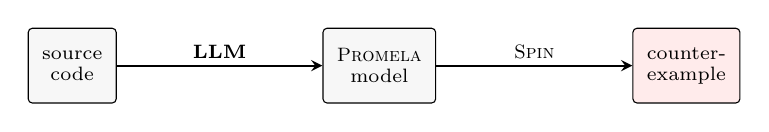
\begin{tikzpicture}[
  font=\scriptsize, >=stealth,
  box/.style={draw, rounded corners=1.5pt, align=center, inner sep=5pt,
              minimum height=0.95cm, fill=black!3},
  lab/.style={font=\scriptsize\bfseries, inner sep=2pt}
]
  \node[box] (code)  at (0,0)    {source\\code};
  \node[box] (model) at (3.9,0)  {\promelaname{}\\model};
  \node[box, fill=red!8] (cex) at (7.8,0) {counter-\\example};

  \draw[->, thick] (code)  -- node[lab, above] {LLM}    (model);
  \draw[->, thick] (model) -- node[lab, above] {\spin{}} (cex);
\end{tikzpicture}

\vspace{1.6cm}

{\normalsize \url{https://spinroot.com}}
\end{center}

\end{frame}
     %  2 min

\end{document}
